\section{Revisão de Bibliográfica}
\vspace*{1cm}
Antes mesmo de introduzir a nossa revisão é bom explicar o que é esse capítulo, a revisão bibliográfica nada mas é que pesquisas sobre determinado assunto, porém que não podem ser realizadas através de qualquer tipo de fonte. Para ser válido, uma
revisão bibliográfica precisa vir de fontes como livros, publicações científicas, fontes seguras onde o autor possui algum tipo de formação sobre aquele determinado
caso que esta sendo pesquisado.

\subsection{Sistema de Informação}
  
Sistema de Informação é um sistema que tem como elemento principal a informação. Tem por objetivo armazenar e fornecer informações, e do mesmo modo a apoiar processos e funções de uma organização. 
Ele é composto por dois subsistemas, social e automatizado.

De forma que, o primeiro inclui pessoas, processos, documentação e informações, e no segundo compõe-se de máquinas, computadores e redes de comunicação, que interligam os elementos ao subsistema social. 

Pode-se dizer que este sistema é maior que um software, pois inclui não só o hardware e software, como também pessoas e agentes que executam os processos fora da máquina, o que mostra que pessoas que não utilizam os computadores também fazem parte deste sistema, e que, consequentemente, necessitam ser observadas e guiadas pelos processos de planejamento e análise de sistemas. 

Por tanto, podem-se ser utilizados vários tipos de sistema de informação nas organizações, classificados de acordo com suas necessidades e tipos de informação.
 \begin{figure}[!h]
	\centering
	\caption{Representação gráfica}
	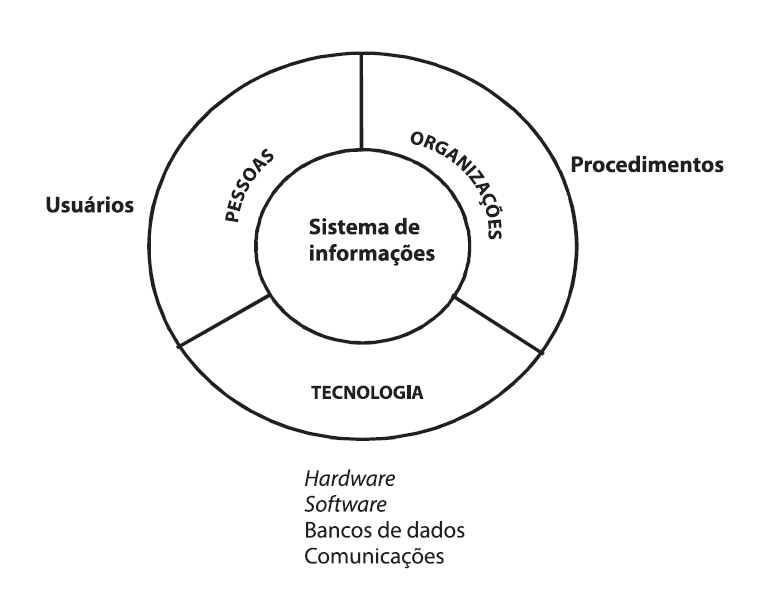
\includegraphics[width=300px, height=200px]{./images/2-1.png}
	\par{Autor(a): Desconhecido}
\end{figure}
\subsubsection{Sistema Transacional}

Um dos tipos de sistemas de informação seria o transacional. Podemos dizer que um sistema transacional é o coração da maior parte das negociações de uma organização. Este sistema oferece uma grande eficiência no ramo empresarial, pois concede suporte às monitorações e às realizações, gerando e armazenando um grande fluxo de dados sobre as negociações. Podemos dizer que o sistema transacional é o sistema operacional das empresas, se caracterizando pela sua alta taxa de atualização, pelo grande volume de dados, por sua precisão e sua pontualidade no decorrer dos processos.

Ou seja, sistemas transacionais são sistemas de suporte às atividades do dia a dia, utilizados em tarefas repetitivas, como, por exemplo, sistemas em geral relacionados à área administrativa-financeira, tais eles como, sistemas contábeis, sistemas de folha de pagamento, sistemas de faturamento, sistemas de compras e sistemas de estoque. Eles, em geral podem ser responsáveis pela coleta e entrada de dados, processamento e armazenamento, e geração de documentos e relatórios.
\subsection{Análise de Requisitos}

Primeiramente é preciso compreender o que é um requisito e qual é a importância de se fazer uma análise e gestão de requisitos. Seu entendimento faz com que o projeto tenha um ponto de partida, de forma que se tenha a definição inicial do sistema para que no final tenha-se atendido aquilo que o cliente necessitava. De acordo com o que (\cite{machado-2011}), em seu livro: “Os requisitos expressam as características e restrições de um produto de software do ponto de vista de satisfação das necessidades do usuário e, em geral, independem da tecnologia empregada na construção da solução, sendo a parte mais crítica e propensa a erros no desenvolvimento de software.” 

De acordo com IEEE (Instituto de Engenheiros Eletricistas e Eletrônicos), sobre Engenharia de Requisitos de Sistemas e de Software, a definição de requisito é, por exemplo, condição ou capacidade necessária para um usuário poder resolver um problema ou atingir um objetivo. Ou, condição ou capacidade que deve ser alcançada por um sistema para ter a necessidade atingida.

Com o conhecimento de um requisito fica mais fácil entender o processo por completo, pois o conjunto de requisitos é necessário para que o software tenha toda capacidade de ajudar o usuário a atingir seus objetivos ou atender sua necessidade. Porém, somente isso não basta, é preciso compreender o usuário e ter a experiência para distinguir quando o cliente realmente quer algo ou não, precisa ter um alinhamento efetivo do que vai ser elaborado e, em caso de positivo e atendendo as requisições, desenvolvido. Entendendo todo o negócio do cliente, como funciona, quais informações são relevantes ou não, tudo isso é de extrema importância para que se tenha bons resultados.

De acordo com (\cite{machado-2011}) análise de requisitos: “São todas as atividades realizadas para identificar, analisar, especificar e definir as necessidades de negócio que um aplicativo deve prover para solução do problema levantado. Requisitos que não refletem as reais necessidades dos usuários, incompletos e/ou inconsistentes, mudanças em requisitos que já foram previamente acordados e a dificuldade para chegar a um acordo entre profissionais de T.I. e usuários são os maiores problemas enfrentados no grupo de atividades de especificação de requisitos.” 

Também explica que após ter a análise dos requisitos, é de suma importância ter a gestão: “Preocupa-se com a documentação, versionamento, controle de mudanças e qualidade dos requisitos levantados na fase de especificação de requisitos. Todo requisito apresenta um ciclo de vida único que acompanha a dinâmica dos negócios associados. Assim sendo, não se pode esperar que um requisito seja imutável ao longo do tempo, uma vez que o negócio do qual o requisito se desprende é dinâmico.”

Os requisitos são variáveis. Podendo ser tanto algo mais simples, quanto funcionalidades básicas de um sistema, quanto mais complexo, como processo de importação com suas taxas cambiais. Independentemente do tipo de funcionalidade, eles podem ser classificados em diferentes níveis, sendo para atingir necessidades e características. A primeira tem como objetivo os problemas no negócio, pessoas ou operacionais que precisam ser encaminhadas para terem um porquê de ser desenvolvido um sistema. Já a segunda é por meio de observação, no qual o sistema satisfaz as necessidades. 

Para o analista responsável por essa tarefa, é preciso ter o domínio e entendimento de requisitos e, saber observar o cliente e todo o processo, para classificar se as atividades são coerentes com os requisitos. 

Quando há muitos clientes em um mesmo projeto, poderá ter conflitos de requisitos, assim, o analista precisa antecipar e evitar os conflitos que podem ocorrer durante o processo, além de definir quais requisitos possuem prioridade e que irão atender o cliente. Por fim, é preciso que tenha uma verificação dos requisitos, que vai definir, de acordo com o cliente, se estão completos e consistentes para o sistema.

\begin{figure}[!h]
	\centering
	\caption{Processo de levantamento e análise de requisitos }
	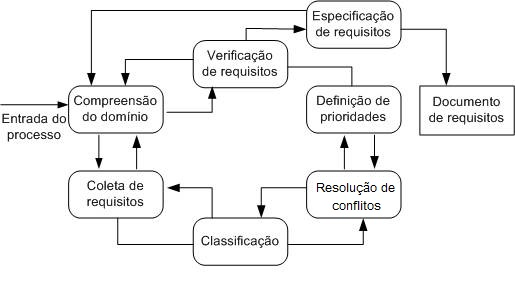
\includegraphics[width=300px, height=200px]{./images/2-10.jpg}
		\par{Autor(a): \cite{sommerville}}
\end{figure}

Para que sejam atingidos tais requisitos é importante seguir um modelo de processo, que é uma junção estruturada de elementos que descrevem processos efetivos, sendo usados para definir objetivos e prioridades onde o foco é a melhoria do processo. Contudo, a qualidade de um sistema é, em grande parte, definido pela qualidade do processo usado.

De modo geral, os requisitos tendem a ser divididos em dois grupos: Requisitos Funcionais e Requisitos Não Funcionais.

\subsubsection{Requisitos Funcionais}

Os Requisitos Funcionais são responsáveis por descrever o comportamento do sistema, as funcionalidades que o sistema possa fornecer. Dependendo do software que for desenvolvido para o cliente, é preciso verificar se os requisitos para esse sistema estão de acordo com as necessidades específicas que o cliente queria que fossem atingidas. As especificações de um requisito funcional são o que vão designar o caminho pelo qual o software desenvolvido vai fazer, sem precisar que o usuário fique esperando para solicitar modificações, de forma que sinta-se efetivamente atendido.

\subsubsection{Requisitos Não Funcionais}

Os Requisitos não Funcionais não exercem as funções de um Requisito Funcional, mas, por outro lado, se atenta em fornecer a melhor qualidade, como passar um sistema com confiabilidade, desempenho, segurança, integridade, entre outros. São responsáveis por definir se o sistema é eficiente ou não para fazer o que se propôs a ser criado, de forma que caso não corresponda com o que foi solicitado, será descartado. De acordo com (\cite{machado-2011}) “Um exemplo de requisito não funcional: A base de dados deve ser protegida para acesso apenas de usuários autorizados.”

\subsubsection{Regras de Negócio}
Regras de Negócio são o que definem a forma da empresa fazer negócio, onde é executado as atividades que compõe o seu serviço ou produto. Os requisitos vem por meio da observação de cada parte do negócio do cliente. A formalização dessa etapa é por um documento que se reúne todas as normas e processos da organização. Para que a observação seja válida, é importante que quem estiver fazendo-a seja alguém que tenha experiência técnica com regras de negócios e processos, pois muitas vezes necessitam de linguagem técnica referente ao negócio.
(\cite{tecnicas-levantamento})

\subsection{Portais web}
Antes de se entrar no assunto propriamente dito, Portais Web, precisa-se entender o conceito de portais.
Portais, que muitas vezes pode ser associado como um sinônimo de site, não o é. Diferentemente dos sites, que têm como foco a acessibilidade e organização de um conteúdo, os portais tem como foco seu público, ou seja, para quem se destina a informação. Assim, apesar de também promoverem a construção de conhecimento, eles têm uma maior sensibilidade para com o leitor.

\subsubsection{Portais de informação}

O termo “portal” foi criado pelos norte-americanos, e só então começou a ser usado no Brasil no ano de 1988.

Os portais de informação podem ser definidos como páginas na internet que possuem uma grande quantidade de informações sobre temas e assuntos, de modo com que as pessoas consigam ter acesso a essa informação. Esses portais são de cunho público, ou seja, qualquer um que deseja saber sobre determinado assunto tratado pelo portal tem livre acesso.

Alguns exemplos de portais são: G1, Estadão e Terra. Todos esses são exemplos de portais de notícias, que são atualizados todos os dias, disponibilizando assim conteúdo novo e atualizado todos os dias para os usuários que desejem saber as notícias do dia, a qualquer momento e em qualquer lugar.

Mas além de portais atualizados diariamente, como os portais de notícias, existem portais que são atualizados periodicamente, pois nestes casos não existe a exigência de uma atualização frequente.
 \begin{figure}[!h]
	\centering
	\caption{Variedade de portais disponíveis}
	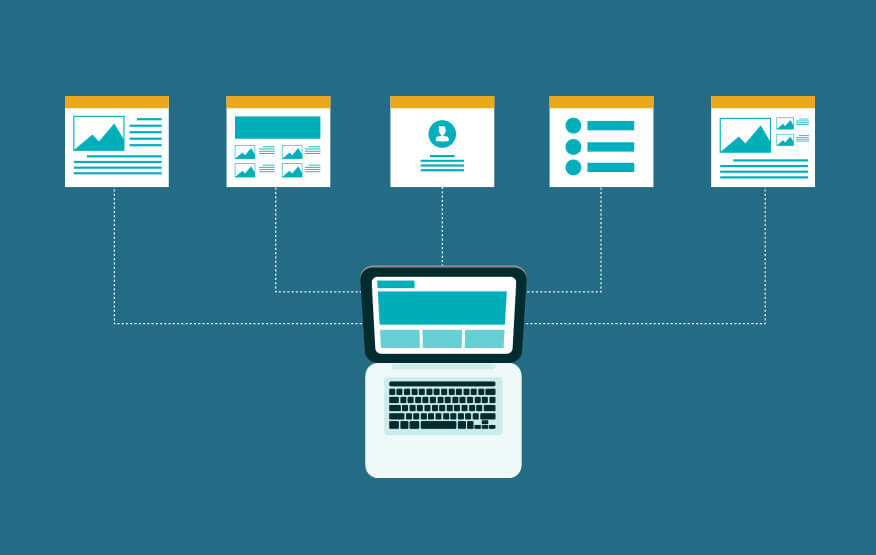
\includegraphics[width=300px, height=200px]{./images/2-3.jpg}
		\par{Autor(a): \cite{loba}}
\end{figure}
\newpage

\paragraph{A importância e a responsabilidade dos portais de informação}\mbox{}\\
\par
Os portais de informação têm como objetivo transmitir as informações propriamente ditas aos usuários, independe do seu tema ou conteúdo. Porém, ser o administrador de um portal requer um alto grau de responsabilidade, pois as informações contidas em um portal podem servir como base de conhecimento para outras pessoas, e, caso o tema não tenha sido bem elaborado, os usuários podem interpretar de maneira errônea as informações contidas no portal, fazendo assim com que um conhecimento “errado” seja transmitido.

\paragraph{A importância e a responsabilidade dos portais de informação}\mbox{}\\
\par
Na internet existe uma “teia” imensa de portais, de diversos temas e assuntos. É importante que exista esta variedade de portais pela web, pois assim um rico conhecimento é gerado e armazenado de forma que as pessoas possam ter acesso por muito tempo.

A interconexão é algo que vale a pena ser estudada, para que uma navegação pelo conteúdo desejado seja mais fluida. Ao acessar um portal sobre um determinado assunto, aquele portal direcionará o usuário a um outro portal de assunto similar, criando assim uma interligação entre os portais peça web, que acarretara em uma cadeia continua de conhecimento específico.

Dessa forma pode-se ver o quão rica em conhecimento a internet pode ser, através de seus portais.

\paragraph{Portais Horizontal e Vertical}\mbox{}\\
\par
Os portais podem ser classificados em horizontais e verticais. O primeiro é mais antigo, dominando a internet principalmente em 1998 a 2000. Já o segundo nasceu no meio deste período de dominância do primeiro, em 1999.

Os portais horizontais fornecem uma leitura mais limpa e de fácil compreensão, não necessariamente no sentido de que usa palavras e linguagem mais simples, mas sim de que visualmente são mais fáceis de se ler e encontrar informações. Dificilmente são usadas frases ou palavras entre aspas e tem entrevistados defendendo uma opinião. Seu foco é a disseminação de informações, o que de certa forma contribui para a formação de leitores passivos, que leem sem se aprofundarem no assunto.

Os portais verticais, diferente dos horizontais, tem como público alvo usuários que se interessam por conteúdo e serviços personalizados. Assim, com este foco, os torna mais únicos, de forma que se tem um aumento nas chances de um usuário voltar a um mesmo portal. Eles surgiram como uma alternativa das empresas de mídia, para que estas não ficassem em desvantagem contra os maiores sites horizontais, que detinham um maior número de tráfego, e consequentemente maiores investimentos dos anunciantes, já que um maior número de tráfego representava uma maior acessibilidade e visibilidade para um anúncio contido neles.

\subsubsection{Sites Institucionais}
Os sites institucionais são com o próprio nome diz, site para instituições. São extremamente importantes atualmente no mercado. Com o grande avanço da internet, é praticamente indispensável que uma instituição possua um site com conteúdo próprio.

Atualmente, praticamente todas as pessoas têm acesso à internet, seja de um smartphone ou de um computador. Sendo assim, quando uma pessoa tem interesse em alguma instituição por algum motivo, a primeira coisa que é feito é uma busca na internet sobre a mesma.

Disponibilizando informações sobre uma instituição na internet, o conhecimento sobre a existência da mesma se torna muito maior em meio a sociedade, tornando o site institucional a porta de entrada das pessoas à instituição.
 \begin{figure}[!h]
	\centering
	\caption{Possibilidades de um site institucional }
	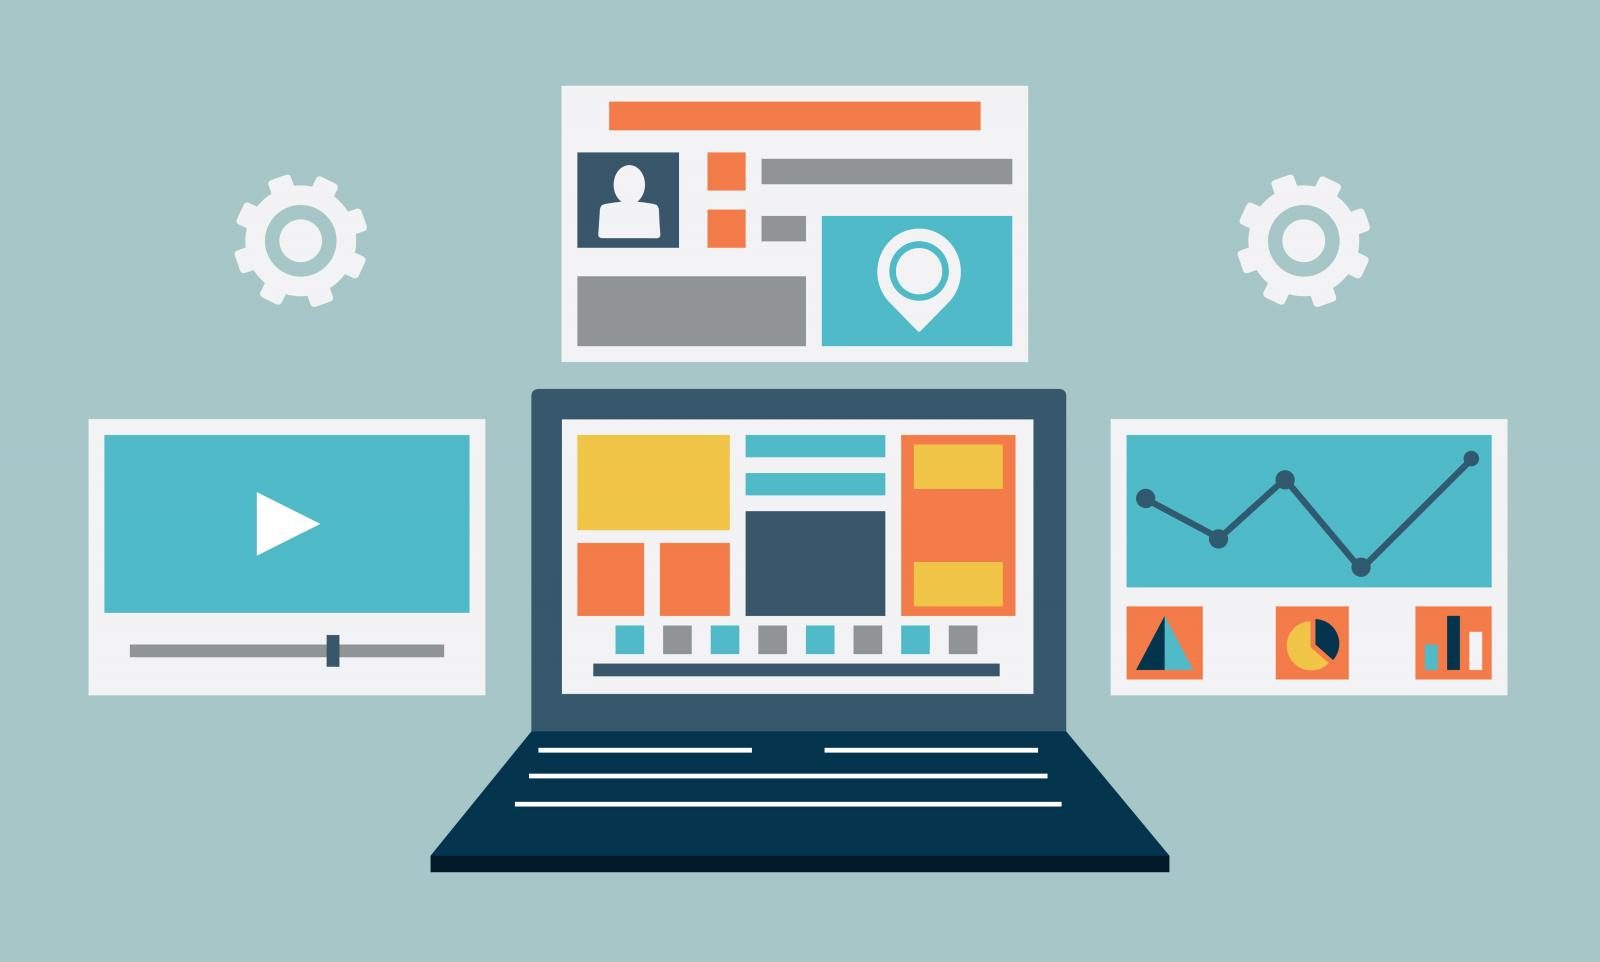
\includegraphics[width=300px, height=200px]{./images/2-4.jpg}
	\par{Autor(a): \cite{markeninja}}
\end{figure}

\paragraph{A importância dos sites institucionais}\mbox{}\\
\par
Como já dito anteriormente, o site institucional é indispensável para qualquer tipo de instituição, seja ela com fins lucrativos ou não.

Este tipo de site gera uma grande visibilidade para a instituição, fazendo com que cada vez mais pessoa conheçam a mesma.

Além da visibilidade, um site agrega muito valor para uma instituição, pois além de disponibilizar informações e recursos para os usuários, mostra seriedade e compromisso com o cliente por parte da instituição.

\subsubsection{Portais Web}

Atualmente os portais web detém uma porcentagem muito grande do conhecimento buscado pela sociedade. A internet teve e tem cada vez mais um papel importantíssimo na sociedade moderna: o compartilhamento de informações.

Existe uma vasta variedade de portais web, possibilitando com que pessoas tenham acesso às informações que antes dificilmente era possível.

E é através destes portais que o mundo se comunica, possibilitado a troca de informação diariamente pelas pessoas.
\newpage
 \begin{figure}[!h]
	\centering
	\caption{Facilidade dos portais web}
	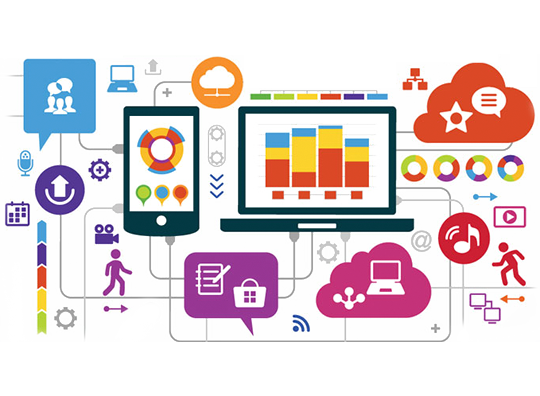
\includegraphics[width=300px, height=200px]{./images/2-5.png}
	\par{Autor(a): \cite{newtechs}}
\end{figure}

\subsubsection{Negócio eletrônico}

O negócio eletrônico, ou como também é conhecido, E-business, é uma das partes mais importantes na internet atualmente.

O E-business trata toda a parte de negócios na web, desde o contato entre empresas, ou entre empresa e cliente até a transação final de valores.

É através deste tipo de negócio que as empresas atuais estão crescendo e se desenvolvendo cada vez mais, agilizando e otimizando seus fluxos de trabalho, fazendo assim com que o lucro adquirido seja muito mais significativo em relação ao limitado meio físico de negócio. Porém, o meio físico não é descartado nesse tipo de negócio eletrônico, apesar da maior parte das etapas do negócio ser feita virtualmente.

 \begin{figure}[!h]
	\centering
	\caption{Melhores resultados com o comercio eletrônico}
	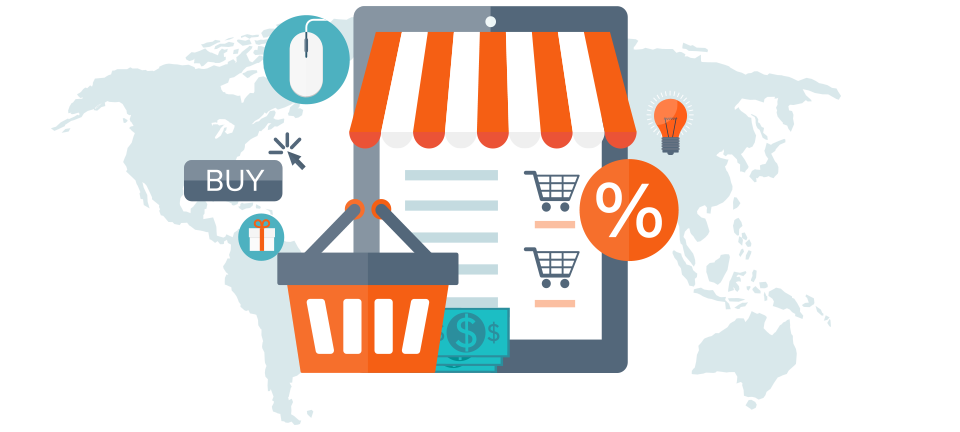
\includegraphics[width=300px, height=150px]{./images/2-6.png}
	\par{Autor(a): \cite{3webbox}}
\end{figure}
\newpage

O e-commerce também está dentro do e-business, sendo uma de suas partes mais importantes, pois é ela que está possibilitando que o mercado consiga atingir metas com muito mais eficiência do que com os métodos padrões presenciais de compra e venda.

Dificilmente nos dias atuais uma pessoa sai de casa para comprar algo, como um eletrodoméstico, eletroeletrônico ou até mesmo roupas. Se tornou muito mais cômodo e prático realizar as compras através da internet, pois com poucos cliques é possível realizar uma compra, com a vantagem de nem se quer precisar sair de casa para ter o produto adquirido.

Outro ponto do negócio eletrônico que tem crescido fortemente é o negócio de produtos usados. Com a facilidade de qualquer pessoa poder anunciar um produto pra venda na internet, muitas vendas são realizadas por dia, por pessoa que não necessariamente sejam pessoas jurídicas, mas sim pessoas físicas.

A dificuldade para achar compradores para um produto usado já não existe mais, fazendo com que seja muito mais fácil e prático achar um comprador.

Algumas das principais modalidades de relacionamento pelas quais o comércio eletrônico pode ser classificado são: B2B, B2C, C2B, B2E e E2B.

\paragraph{B2B}\mbox{}\\
\par
B2B (Business to Business) seria basicamente a relação entre empresas, podendo ser através da troca de serviços e/ou informações entres elas. Exemplo: uma empresa e seu fornecedor.

\paragraph{B2C}\mbox{}\\
\par
B2C (Business to Consumer) não é apenas a relação de uma empresa com um consumidor, mas também pode ser com um cliente. Exemplos: empresa vendendo um produto para um consumidor, ou um serviço para um cliente.

\paragraph{C2B}\mbox{}\\
\par
C2B (Consumer to Business) é basicamente o contrário da anterior, no sentido da transação. É quando um cliente ou consumidor fornece informações para uma empresa. Exemplos: cadastro de currículos em um site de uma empresa, ou sugestões e avaliações dos serviços oferecidos ou atendimento de uma empresa.


\par
B2E (Business to Employee) é a relação de uma empresa com seus funcionários. Podendo ser tanto treinamentos ou serviços oferecidos pela empresa para seus funcionários, quanto na aquisição de algum produto ou serviço da empregadora como um cliente final, mas com algumas condições especiais, como desconto para funcionários, mas com uma cota por mês.

\paragraph{E2B}\mbox{}\\
\par
Por fim, E2B (Employee to Business) é o contrário da anterior, no sentido da transação. Lembra um pouco o C2B, mas em vez do consumidor/cliente estar fornecendo informações, é um funcionário da própria empresa que o faz. Exemplo: Um funcionário faz uma sugestão de como melhorar algum setor da empresa.
 \begin{figure}[!h]
	\centering
	\caption{Modalidades de relacionamento}
	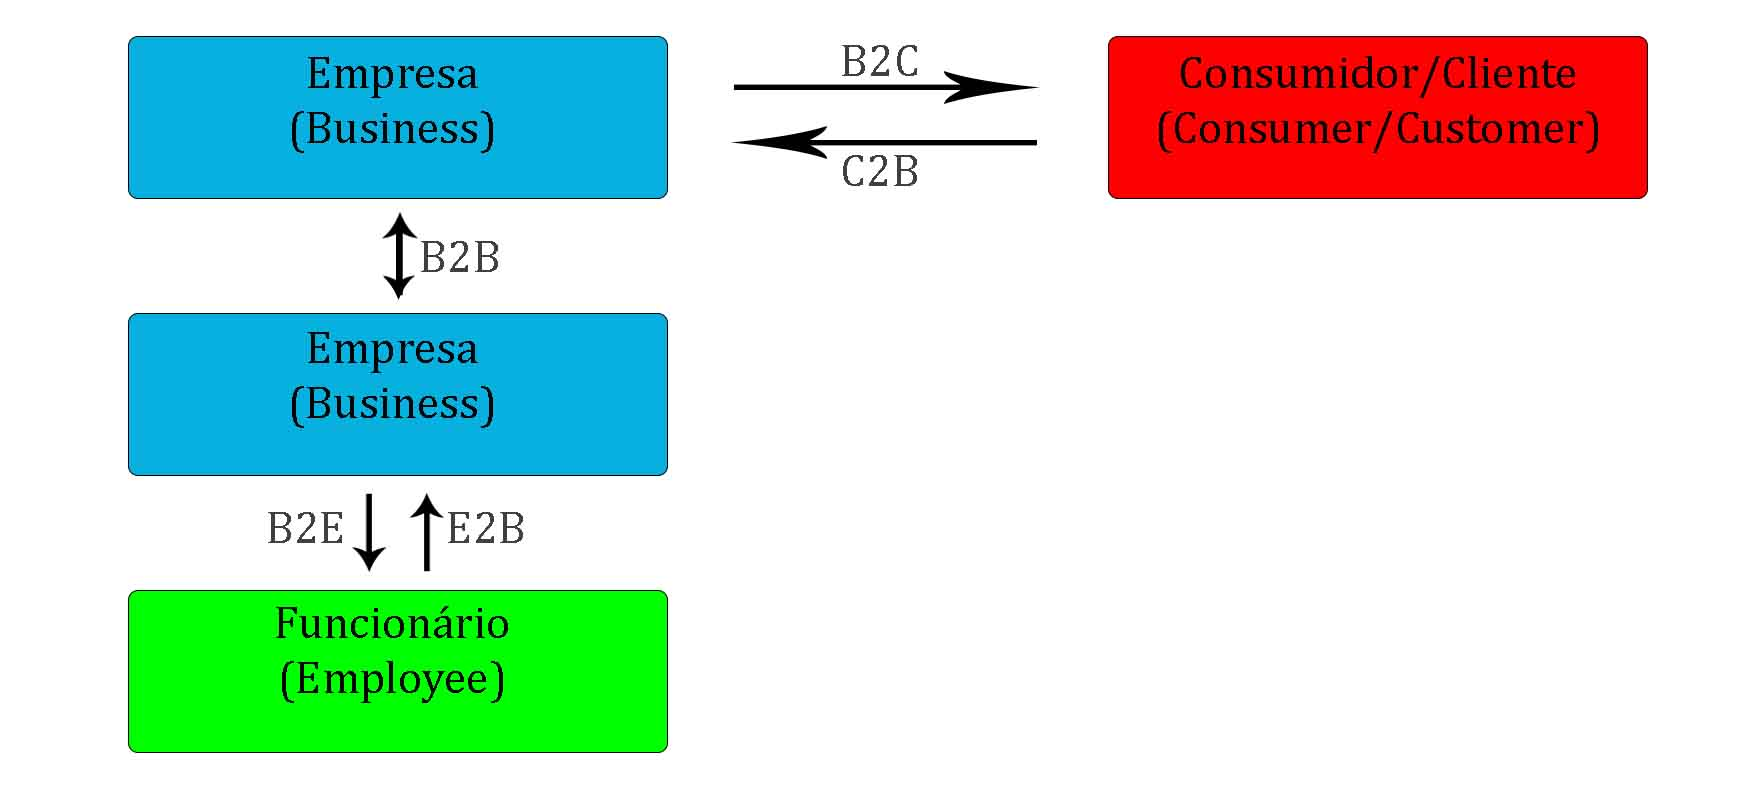
\includegraphics[width=300px, height=200px]{./images/2-7.jpg}
	\par{Autor(a): Letícia Sayuri Fujimori}
\end{figure}

\subsection{Aplicativos Mobile}
Os aplicativos estão cada vez mais sendo usado pelas pessoas, tendo um papel muito importante na vida delas, facilitando diversas atividades.

Com o aumento dos smartphones os apps consequentemente ganham muita credibilidade, pois com maior número de smartphones para que pessoas tenham acesso aos aplicativos, maior procura e a quantidade de aplicativos que são lançados.

O Brasil, segundo o ranking da Flurry, está na decima colocação entre países que utilizam aplicativos tanto no Android como no iOS.

De acordo com Brookshear [1997], "aplicativo de software consiste de programas que executam tarefas específicas para utilização em máquinas. Exemplos de aplicativos de software incluem planilha eletrônica, sistemas de banco de dados, sistemas de editoração eletrônica, programas de desenvolvimento de software e jogos."

Aplicativos mobiles são softwares que tem como objetivo o funcionamento em smartphones e tablets, tendo nestes seu melhor desempenho. Sendo através de uma “loja” onde se tem aplicativos como app store ou Android Market que as pessoas tem acesso ao download do aplicativo.
Aplicativos mobile tem seus prós e contras, apesar de serem muito benéficos a comunidade, ainda trazem seus problemas, mas que não causam tanto impacto.

\subsubsection{Vantagens dos dispositivos mobile}
Baixo custo ou até mesmo sem custo para serem usados. A interface é adaptada para o dispositivo e tem um trafego de dados que é menor comparando ao uso de navegadores.

Tem uma facilidade de uso altíssima que possibilita o usuário a ter uma experiencia melhor, com uso de recursos e interfaces de dispositivos que otimizam a navegação e a agilidade.

Alguns aplicativos possuem acesso offline, e isso possibilita uma navegação sem internet fazendo com que pessoas consigam ter uma experiencia ainda melhor caso esteja sem internet.

\subsubsection{Desvantagem dos dispositivos mobile}
Aplicativos tem muitas atualizações de versões de acordo com as versões dos smartphones ou tablets que vão sendo lançados, para melhorar o aplicativo e trazer novos recursos ao app. Porém, com isso temos alguns problemas, como a compatibilidade do smartphone, algumas atualizações fazem com que o smartphone perca a compatibilidade com o app, pois ficou mais pesado ou não roda mais por algum motivo.

Na parte de aplicativos mobile temos diversos tipos de aplicativos, entre eles: serviços, informações, comunicação, entretenimento, entre outros. Serviços nos fornecem informações e conteúdo de um modo mais simples e ágil, como aplicativos que verificam o tempo, navegação de mapas ou solicitações de resgates de seguradores de carro como exemplo.

Em relação aos tipos mencionados, os de informações são para os acessos a conteúdos que são constantemente atualizados, sendo que as atualizações são feitas em tempos reais, como em telefones, promoções, consulta de produtos, entre alguns outros.

Na parte da comunicação o aplicativo permite uma conexão entre as pessoas, como um Skype, WhatsApp, Messenger entre outros. Já na questão do entretenimento são aplicativos que levam a diversão para o público em geral, como jogos que são extremamente intuitivos.

Na parte de aplicativos temos tanto aplicativos nativos como aplicativos híbridos. Aqueles consistem em aplicativos que funcionam somente em Android ou somente em IOS, estes funcionam tanto em Android quanto em IOS.

\subsubsection{Nativo}
Aplicativos nativos são desenvolvidos para serem usados em uma plataforma apenas, como por exemplo somente no Android, sendo capaz de fazer e explorar as funções da plataforma em questão. Aplicativos nativos conseguem explorar todo o potencial do dispositivo como a câmera fotos, GPS, entre outros.

Um aplicativo nativo seria todo programa construído sob medida para uma plataforma, com a intenção de funcionar em sintonia com o dispositivo e suas especificidades.

Os apps nativos funcionam de uma forma mais prática, respondendo todos os comandos a que são propostos sem dificuldades. Mesmo que a estrutura de um programa nativo seja trabalhosa, eles são bem estáveis, pois não precisam de internet para serem usados, tornando a experiência e prática mais independentes e livres de perdas caso fiquem sem conexão.

Eles são mais completos e dinâmicos por serem desenvolvidos exatamente para ser aproveitado o máximo da plataforma na qual foram criados.

\subsubsection{Híbridos}
Aplicativos híbridos são parte nativos e parte mwa (Mobile Web Aplication).  Os aplicativos híbridos são iguais aos nativos em alguns quesitos, devem ser baixados através de um app de loja, ficam armazenados na tela principal do dispositivo e pode usar todas as funcionalidades do dispositivo como o gps, a câmera. Apps híbridos podem ter sua base em html5 e serem exibidos através de um navegador embutido no aplicativo, tendo parte ou tudo carregado na web.

Aplicativos híbridos são famosos, pois permitem o desenvolvimento em várias plataformas utilizando o mesmo html para vários sistemas, como IOS, Android.

A maior vantagem de um aplicativo híbrido seria sua compatibilidade com os SOs. Caso queira desenvolver de forma híbrida em android e quiser expandir para windowsPhone, terá de reescrever seu código para IOS, com o desenvolvimento híbrido um código pode ser compilado para várias plataformas, deixando assim mais prático e econômico.


\normalsize{\textbf{Augusto Cesar Scafi 2º Semestre, Hakawã Alves 2º Semestre, Letícia Sayuri Fujimori 2º Semestre, Lilian de Oliveira 2º Semestre, Vinicius Matos de Souza 1º Semestre, Vitor Dueñas Santana Morais 2º Semestre}}

\newpage 